\documentclass[dvisvgm,hypertex,aspectratio=169]{beamer}
\usefonttheme{serif}

\usepackage[draft]{animate}
\usepackage{ifthen}


%%%%%%%%%%%%%%%%%%%%%%%%%%%%%%%%%%%%%%%%%%%%%%%%%%%%%%%%%%%%%%%%%%%%%%%%%%%%%%%
% PageDown, PageUp key event handling; navigation symbols
%%%%%%%%%%%%%%%%%%%%%%%%%%%%%%%%%%%%%%%%%%%%%%%%%%%%%%%%%%%%%%%%%%%%%%%%%%%%%%%
\usepackage[totpages]{zref}
\usepackage{atbegshi}
\usepackage{fontawesome}
\setbeamertemplate{navigation symbols}{}
\AtBeginShipout{%
  \AtBeginShipoutAddToBox{%
    \special{dvisvgm:raw
      <defs>
      <script type="text/javascript">
      <![CDATA[
        document.addEventListener('keydown', function(e){
          if(e.key=='PageDown'){
            \ifnum\thepage<\ztotpages
              document.location.replace('\jobname-\the\numexpr\thepage+1\relax.svg');%
            \fi
          }else if(e.key=='PageUp'){
            \ifnum\thepage>1
            %document.location.replace('\jobname-\the\numexpr\thepage-1\relax.svg');%
              document.location.replace('\jobname-\makeatletter\@anim@pad{2}{\thepage-1}\makeatother\relax.svg');%
            \fi%
          }
        });
      ]]>
      </script>
      </defs>
    }%
  }%
  \AtBeginShipoutUpperLeftForeground{%
    \raisebox{-\dimexpr\height+0.5ex\relax}[0pt][0pt]{\makebox[\paperwidth][r]{%
      \normalsize\color{structure!40!}%
      \ifnum\thepage>1%
      \href{\jobname-\the\numexpr\thepage-1\relax.svg}{\faArrowLeft}%
      \else%  
        \textcolor{lightgray}{\faArrowLeft}%  
      \fi\hspace{0.5ex}%
      \ifnum\thepage<\ztotpages%
      \href{\jobname-\the\numexpr\thepage+1\relax.svg}{\faArrowRight}%
      \else%
        \textcolor{lightgray}{\faArrowRight}%  
      \fi%
      \hspace{0.5ex}%
    }}%
  }%  
}%
%%%%%%%%%%%%%%%%%%%%%%%%%%%%%%%%%%%%%%%%%%%%%%%%%%%%%%%%%%%%%%%%%%%%%%%%%%%%%%%

\usepackage{tikz}
\usepackage{pgfplots}
\pgfplotsset{compat=1.16}
\usetikzlibrary{calc}
\usepackage{amsmath}
\DeclareMathOperator{\sign}{sgn}


\author{Kjartan Halvorsen}
\date{2021-05-10}
\title{Modelación y automatización}

% ------------------------------------------------
% Determine which slides to include
\includeonlyframes{%
%  A1,%
%  M1,%
%  M2,%
%  M3,%
  M4,%
  M5,%
  M6,%
}
% ------------------------------------------------


\newcommand{\hummeranimation}[1]{%

  \def\velocity{1.5}
  \def\startbrake{3}
  \def\braketimeconst{3}

  \begin{center}

  %\begin{animateinline}[controls,autoplay,loop]{20}
  \begin{animateinline}[ ]{28}
      \multiframe{60}{n=0+0.15}{
        \begin{tikzpicture}
          \useasboundingbox (-1 cm, -1 cm) rectangle (9 cm, 3 cm);
          \pgfmathsetmacro{\xpos}{\velocity*\n*(\n<\startbrake) + (\velocity*\startbrake + \velocity*\braketimeconst*(1-(exp(-(\n-\startbrake)/\braketimeconst))))*(\n >= \startbrake)}

            \node[anchor=south,] at (\xpos cm, 0) {\ifnum#1 > 0 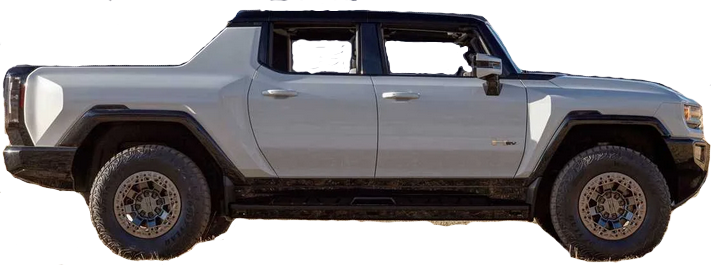
\includegraphics[width=15 mm]{hummer-ev.png} \else \tikz \draw[fill, black] (0,0) rectangle (1,1); \fi};
            \draw[->, black!90, semithick] (-1, 0.16) -- (9 , 0.16) node[below, pos=1] {$X$};
        \end{tikzpicture}
      }
    \end{animateinline}
  \end{center}
}

\begin{document}

\maketitle


\begin{frame}[label=A1]{Un sistema mecánico}

  
  \hummeranimation{1}

  \alert{Actividad} Indica con flechas todas las fuerzas que afectan el coche. 

\end{frame}


\note{%
}

\begin{frame}[label=I1]{Intuición para sistemas mecánicos}

  Un coche va a velocidad constante en una autopista horizontal. En el instante $t=t_1$, el conductor pone la transmisión en 'N', desconectando el motor de las ruedas. Cuál de las siguientes graficas describe mejor la velocidad $v(t)=\dot{X}(t)$ del coche?

  \begin{center}
    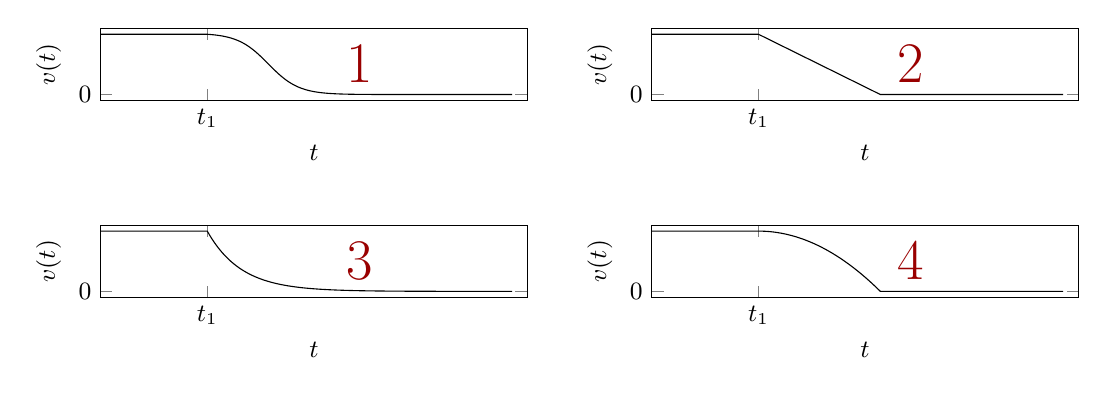
\begin{tikzpicture}
      \small

      \begin{axis}[
        width=7cm,
        height=2.5cm,
        xlabel={$t$},
        ylabel={$v(t)$},
        xmin=-3.5,
        xmax=10.5,
        ytick = {0},
        xtick = {0},
        xticklabels = {$t_1$},
        ]
        \addplot+[black, no marks, domain=-4:10, samples=400,variable=k] { (k < 0) + (k>0)*(1+exp(-4))/(1+exp(4*(0.5*k-1)))};

        \node[black!40!red] at (axis cs: 5, 0.5) {\huge 1};
      \end{axis}

      \begin{axis}[
        xshift=7cm,
        width=7cm,
        height=2.5cm,
        xlabel={$t$},
        ylabel={$v(t)$},
        xmin=-3.5,
        xmax=10.5,
        ytick = {0},
        xtick = {0},
        xticklabels = {$t_1$},
        ]
        \addplot+[black, no marks, domain=-4:10, samples=400,variable=k] { (k<0) + ((k>=0) - (k>4))*(1/4*(4-k)) };
        \node[black!40!red] at (axis cs: 5, 0.5) {\huge 2};
      \end{axis}

      \begin{axis}[
        xshift=0cm,
        yshift=-2.5cm,
        width=7cm,
        height=2.5cm,
        xlabel={$t$},
        ylabel={$v(t)$},
        xmin=-3.5,
        xmax=10.5,
        ytick = {0},
        xtick = {0},
        xticklabels = {$t_1$},
        ]
        \addplot+[black, no marks, domain=-4:10, samples=400,variable=k] { (k<0) + (k>0)*exp(-0.9*k)};
        \node[black!40!red] at (axis cs: 5, 0.5) {\huge 3};
      \end{axis}

      \begin{axis}[
        xshift=7cm,
        yshift=-2.5cm,
        width=7cm,
        height=2.5cm,
        xlabel={$t$},
        ylabel={$v(t)$},
        xmin=-3.5,
        xmax=10.5,
        ytick = {0},
        xtick = {0},
        xticklabels = {$t_1$},
        ]
        \addplot+[black, no marks, domain=-4:10, samples=400,variable=k] { (k<0) + ((k>=0) - (k>4))*(1-1/16*pow(-k,2)) };
        \node[black!40!red] at (axis cs: 5, 0.5) {\huge 4};
      \end{axis}


    \end{tikzpicture}

  \end{center}

\end{frame}

\begin{frame}[label=M1]{Modelación}

  \hummeranimation{1}

  ¿Cómo \alert{modelar} este sistema?

  Depende del \alert{propósito}: ¿Para qué necesitamos el modelo?
\end{frame}

\begin{frame}[label=M2]{Modelación - simplificar}

  \hummeranimation{0} % Just black box

  \begin{center}
    \begin{tikzpicture}
      \node[] (hev) {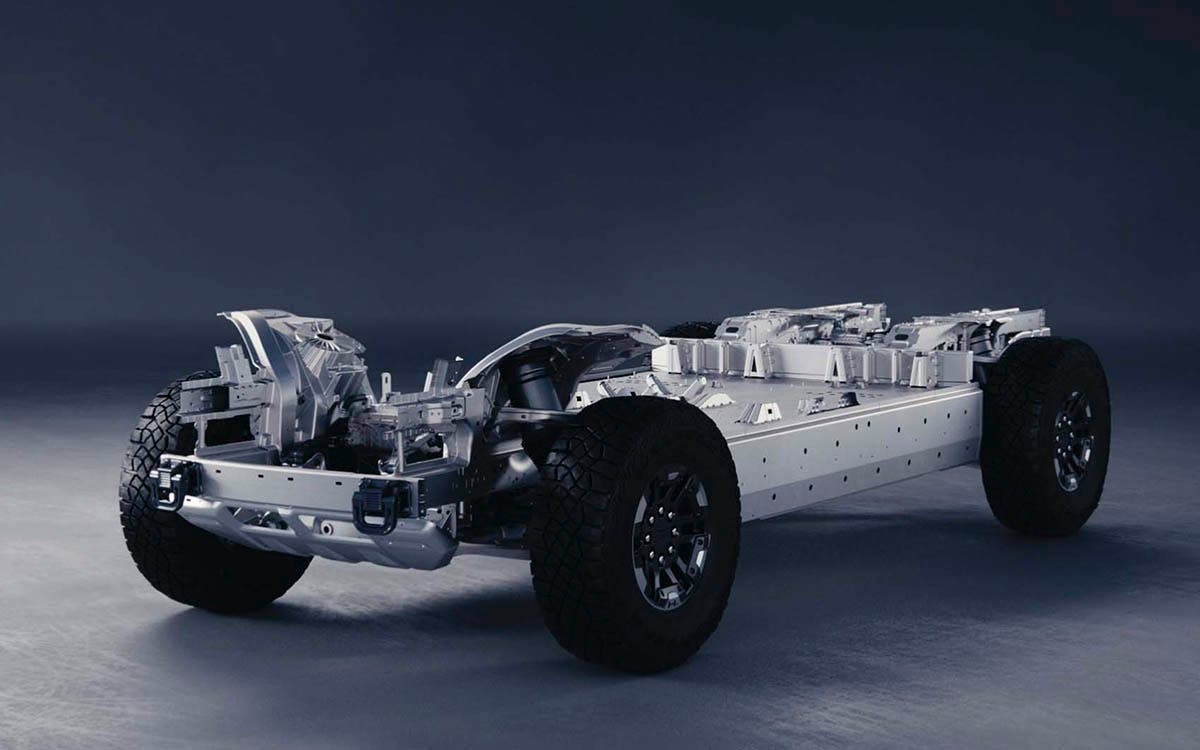
\includegraphics[height=2cm]{hummer-ev.jpg}};
      \node[draw, fill, right of=hev, node distance=2 cm, minimum height=0.3cm, minimum width=0.3cm] (pm) {};

      \draw[thick, ->] (hev) to (pm);
    \end{tikzpicture}
  \end{center}
\end{frame}

\begin{frame}[label=M3]{Modelo de masa puntual}

  La segunda ley de Newton: ``Masa por acceleración es igual a la suma de las fuerzas''
  \[ \frac{d}{dt} (mv) = \sum_i F_i\]
  \begin{center}
    \small 
    \begin{tikzpicture}[scale=1.4, transform shape]
      \node[anchor=south,] at (1, 0) (hummer) {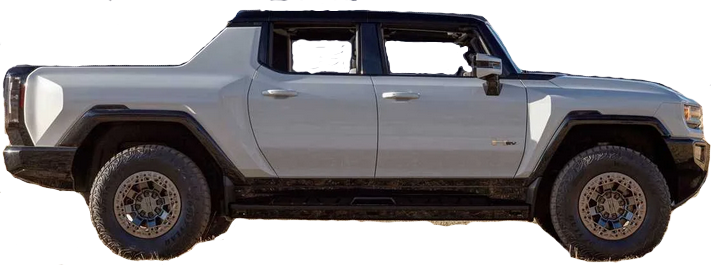
\includegraphics[width=15 mm]{hummer-ev.png}};
      \node[coordinate] (com) at ($ (hummer.center) + (0.15, 0) $) {};
      \node[coordinate] (wheels) at ($ (hummer.south) + (0, 0.16) $) {};
      
      \draw[->, black!90, semithick] (-1, 0.16) -- (9 , 0.16) node[below, pos=1] {$X$};
      \draw[->, black!90, ] (-1, 0.16) -- (-1 , 3) node[left, pos=1] {$Y$};
      
      \draw[thick, green!70!black, ->] (com) -- ++(0, -2cm) node[right] {$F_g = mg$};
      \draw[thick, orange!80!black, ->] (wheels) -- ++(0, 1.3cm) node[right] {$F_{n}$};
      \draw[thick, red!80!black, ->] (wheels) -- ++(2cm, 0) node[below] {$F_m$};
      \draw[thick, blue!80!black, <-] (hummer.east) -- ++(2cm, 0) node[above] {$F_d$};

    \end{tikzpicture}
  \end{center}

  No hay acceleración en la dirección $Y$ (equilibrio en las fuerzas perpendiculares al suelo)
  \[ 0 = F_{n} - F_g \quad \Rightarrow \quad F_{n} = F_g = mg\]
  En la dirección $X$:
  \[ m\dot{v} = F_m - F_d\]
\end{frame}

% Masa puntual?
\begin{frame}[label=M4]{Modelo de masa puntual}
  \[ m\dot{v} = F_m - F_d\]
  Modelo cuadratico del arrastre \(F_d = \sign(v)kv^2\).

\begin{center}
    \begin{tikzpicture}
      \begin{axis}[
        axis lines = middle,
        ytick=\empty,
        xtick=\empty,
        xlabel={$v$},
        ylabel={$F_d$},
        ]
        
        \addplot [blue!80, smooth, domain=-4:4] { sign(x)*x*x};

      \end{axis}
    \end{tikzpicture}
  \end{center}
  \[ m\dot{v} + \sign(v)kv^2 = F_m, \qquad \text{Ecuación diferencial nonlineal}\]
\end{frame}

\begin{frame}[label=M5]{Modelo de masa puntual}
  Assumendo que la fuerza del motor $F_m$ es constante. Cómo se comporta el sistema?
  \[ \dot{v} = \frac{1}{m}(F_m - \sign(v)kv^2)\]
\begin{center}
    \begin{tikzpicture}
      \begin{axis}[
        axis lines = middle,
        ytick=\empty,
        xtick=\empty,
        xlabel={$v$},
        ylabel={$\dot{v}$},
        ymax=5,
        ]
        
        \addplot [orange!80, smooth, domain=0:2.4] {4-sign(x)*x*x};

      \end{axis}
    \end{tikzpicture}
  \end{center}
\end{frame}

\begin{frame}[label=M6]{Modelo de masa puntual}
  \[ m\dot{v} = F_m - F_d\]
  Modelo del arrastre incluyendo resistencia a la rodadura \(F_d = \sign(v)(r + kv^2)\).

\begin{center}
    \begin{tikzpicture}
      \begin{axis}[
        axis lines = middle,
        ytick=\empty,
        xtick=\empty,
        xlabel={$v$},
        ylabel={$F_d$},
        ]
        
        \addplot [blue!80, domain=-4:4, samples=800] { sign(x)*(0.4 + x*x)};

      \end{axis}
    \end{tikzpicture}
  \end{center}
\end{frame}



\begin{frame}[label=M7]{Modelación}
  La segunda ley de Newton: ``Masa por acceleración es igual a la suma de las fuerzas''
  \[ \frac{d}{dt} (mv) = \sum_i F_i,  \qquad \frac{d}{dt}J\omega = \sum_i T_i\] 
  \begin{center}
    \small 
    \begin{tikzpicture}[scale=1.4, transform shape]
      \node[anchor=south,] at (1, 0) (hummer) {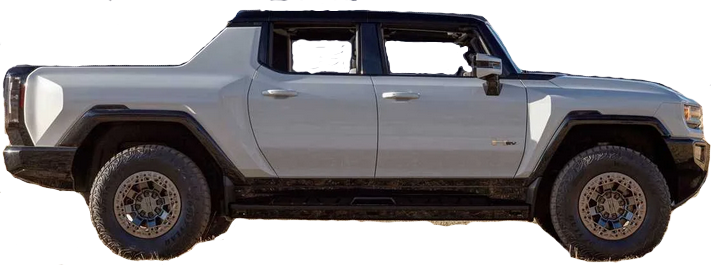
\includegraphics[width=15 mm]{hummer-ev.png}};
      \node[coordinate] (com) at ($ (hummer.center) + (0.15, 0) $) {};
      \node[coordinate] (bw) at ($ (hummer.south) + (-0.42, 0.16) $) {};
      \node[coordinate] (fw) at ($ (hummer.south) + (0.52, 0.16) $) {};
      \node[coordinate] (arrowb) at ($ (bw) + (0, 0.7)$) {};
      \node[coordinate] (arrowf) at ($ (fw) + (0, 0.9)$) {};
      
      \draw[->, black!90, semithick] (-1, 0.16) -- (9 , 0.16) node[below, pos=1] {$X$};
      \draw[->, black!90, ] (-1, 0.16) -- (-1 , 3) node[left, pos=1] {$Y$};
      
      \draw[thick, green!70!black, ->] (com) -- ++(0, -2cm) node[right] {$F_g = mg$};
      \draw[thick, orange!80!black, ->] (fw) -- ++(0, 1.3cm) node[right] {$F_{nf}$};
      \draw[thick, orange!80!black, ->] (bw) -- ++(0, 1.2cm) node[left] {$F_{nb}$};
      \draw[thick, red!80!black, ->] (hummer.south) ++(-0.42, 0.16) -- ++(2cm, 0) node[below] {$F_m$};
      \draw[thick, blue!80!black, <-] (hummer.east) -- ++(2cm, 0) node[above] {$F_d$};

      \draw[<-] (arrowb) -- ++ (-0.5, 0);
      \node at ($ (arrowb) + (0.2, 0.3)$) {$d_b$};

      \draw[<-] (arrowf) -- ++ (0.5, 0);
      \node at ($ (arrowf) + (-0.2, 0.3)$) {$d_f$};
      \draw[thin, dashed] (com) -- ++(0, 15mm);
      \draw[thin, dashed] (com) -- node[coordinate, pos=0.8] (hh) {} ++(-2 , 0);
      
      \draw[<-] ($ (com) + (0, 0.44) $) -- ++ (0.5, 0);
      \draw[<-] ($ (com) + (0, 0.64) $) -- ++ (-0.5, 0);

      \draw[<-] (hh) -- ++ (0, 0.5);
      \draw[<-] (hh |- 0, 0.16) -- ++ (0, -0.5) node[below] {$h$};
      
    \end{tikzpicture}
  \end{center}

  No hay acceleración en la dirección $Y$ (equilibrio en las fuerzas perpendiculares al suelo)
  \[ 0 = F_{nb} + F_{nf} - F_g \quad \Rightarrow \quad F_{nb} + F_{nf} = F_g = mg\]
  En la dirección $X$:
  \[ m\dot{v} = F_m - F_d\]
  Rotación con respeto al centro de masa:
  \[ J\dot{\omega} = F_{nf}d_f - F_{nb}d_b + F_m h\]
  
  
\end{frame}

\begin{frame}[label=M6]{Modelación}
  En estado estable \(\dot{v} = 0\), \(\dot{\omega}=0\).
  
  \begin{center}
    \small 
    \begin{tikzpicture}[scale=1.4, transform shape]
      \node[anchor=south,] at (1, 0) (hummer) {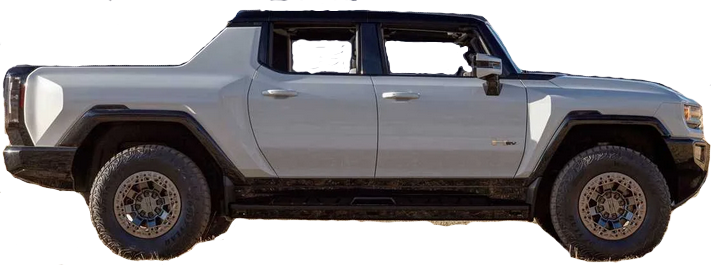
\includegraphics[width=15 mm]{hummer-ev.png}};
      \node[coordinate] (com) at ($ (hummer.center) + (0.15, 0) $) {};
      \node[coordinate] (bw) at ($ (hummer.south) + (-0.42, 0.16) $) {};
      \node[coordinate] (fw) at ($ (hummer.south) + (0.52, 0.16) $) {};
      \node[coordinate] (arrowb) at ($ (bw) + (0, 0.7)$) {};
      \node[coordinate] (arrowf) at ($ (fw) + (0, 0.9)$) {};
      
      \draw[->, black!90, semithick] (-1, 0.16) -- (9 , 0.16) node[below, pos=1] {$X$};
      \draw[->, black!90, ] (-1, 0.16) -- (-1 , 3) node[left, pos=1] {$Y$};
      
      \draw[thick, green!70!black, ->] (com) -- ++(0, -2cm) node[right] {$F_g = mg$};
      \draw[thick, orange!80!black, ->] (fw) -- ++(0, 1.3cm) node[right] {$F_{nf}$};
      \draw[thick, orange!80!black, ->] (bw) -- ++(0, 1.2cm) node[left] {$F_{nb}$};
      \draw[thick, red!80!black, ->] (hummer.south) ++(-0.42, 0.16) -- ++(2cm, 0) node[below] {$F_m$};
      \draw[thick, blue!80!black, <-] (hummer.east) -- ++(2cm, 0) node[above] {$F_d$};

      \draw[<-] (arrowb) -- ++ (-0.5, 0);
      \node at ($ (arrowb) + (0.2, 0.3)$) {$d_b$};

      \draw[<-] (arrowf) -- ++ (0.5, 0);
      \node at ($ (arrowf) + (-0.2, 0.3)$) {$d_f$};
      \draw[thin, dashed] (com) -- ++(0, 15mm);
      \draw[thin, dashed] (com) -- node[coordinate, pos=0.8] (hh) {} ++(-2 , 0);
      
      \draw[<-] ($ (com) + (0, 0.44) $) -- ++ (0.5, 0);
      \draw[<-] ($ (com) + (0, 0.64) $) -- ++ (-0.5, 0);

      \draw[<-] (hh) -- ++ (0, 0.5);
      \draw[<-] (hh |- 0, 0.16) -- ++ (0, -0.5) node[below] {$h$};
      
    \end{tikzpicture}
  \end{center}

  \begin{align}
     0 &= F_{nb} + F_{nf} - F_g \quad \Rightarrow \quad F_{nb} + F_{nf} = F_g = mg\\
     0 &= F_m - F_d\\
    0 &= F_{nf}d_f - F_{nb}d_b + F_m h
 \end{align}
           
    Son tres ecuaciones. Dado la masa $m$,  la gemetría ($h$, $d_f$ y $d_b$) y la fuerza de resistencia $F_d$, se puede despejar las tres fuerzas $F_m$, $F_{nb}$ y $F_{nf}$.
    
  
\end{frame}

\note{%
  - Multiply (1) by d_b and add to (3)
    0 = F_{nb} + F_{nf} - F_g
    0 = F_m - F_d
    0 = F_{nf}d_f - F_{nb}d_b + F_m h + F_{nb}d_b + F_{nf}d_b - mgd_b = F_{nf}(d_f+d_b) + F_m h - F_gd_b
  - Solve (3) for F_{nf}
     F_{nf} = (-F_d h + F_g d_b)/(d_f + d_b)
  - Substitute result in (1)
    F_{nb} = F_g - F_{nf} = F_g (d_f + d_b)/(d_f + d_b) - (-F_d h + F_g d_b)/(d_f + d_b)
           = (mg d_f + F_d h)/(d_f + d_b)  


           Pregunta extra. m=5000kg, d_f = 1.6m, d_b = 1.8m, and h=0.7m
           A que fuerza del motor F_m se pierda el contacto?
           
           
}



\end{document}
